\documentclass[11pt,a4paper,parskip=half]{scrartcl}

\usepackage[utf8]{inputenc}
\usepackage[T1]{fontenc}
\usepackage{lmodern}
\usepackage[french]{babel}
\usepackage{microtype}
\usepackage{xcolor}
\usepackage{booktabs}
\usepackage{tabularx}
\usepackage{array}
\usepackage{enumitem}
\usepackage{graphicx}
\usepackage{listings}
\usepackage{setspace}
\usepackage[colorlinks=true,linkcolor=darkgray,urlcolor=certgreen!70!black]{hyperref}

\definecolor{certgreen}{HTML}{22C55E}
\definecolor{darkgray}{HTML}{1F1F1F}
\definecolor{rowgray}{HTML}{F6F8F6}
\definecolor{codebg}{HTML}{F3F5F3}

\setkomafont{title}{\bfseries\LARGE\color{darkgray}}
\setkomafont{subtitle}{\large\mdseries\color{darkgray!70}}
\setkomafont{section}{\bfseries\Large\color{darkgray}}
\setkomafont{subsection}{\bfseries\large\color{darkgray}}
\RedeclareSectionCommand[beforeskip=1.4em,afterskip=0.5em]{section}
\RedeclareSectionCommand[beforeskip=0.9em,afterskip=0.3em]{subsection}

\setlength{\parindent}{0pt}
\setlength{\emergencystretch}{2em}
\setstretch{1.06}
\setlist{leftmargin=1.2em,itemsep=2pt,parsep=2pt}
\graphicspath{{../screenshots/}}

\lstdefinestyle{solidity}{
  basicstyle=\ttfamily\footnotesize,
  backgroundcolor=\color{codebg},
  frame=single,
  framerule=0.4pt,
  rulecolor=\color{darkgray!25},
  xleftmargin=0.8em,
  xrightmargin=0.8em,
  breaklines=true,
  columns=fullflexible,
  keepspaces=true,
  showstringspaces=false,
  aboveskip=0.8em,
  belowskip=0.8em,
}
\lstset{style=solidity}

\title{Devoir 2 --- Migration du registre vers ERC-721}
\subtitle{OpenZeppelin, rôles, métadonnées on-chain et audit}
\author{Yassi}
\date{Novembre 2026}

\begin{document}

\maketitle

\begin{quote}
\small
Le registre du Devoir 1 remplissait son rôle, mais il ne produisait pas un token
standard. Celui-ci est repris ici sous forme d'ERC-721 : un \texttt{tokenId} par
certificat, des métadonnées lisibles par un wallet, et des rôles explicites pour
séparer l'émission de l'administration.
\end{quote}

\section{Passage à l'ERC-721}

{\footnotesize
\texttt{CertificateNFT} hérite de \texttt{ERC721URIStorage}, \allowbreak
\texttt{AccessControl}, \allowbreak \texttt{Pausable} et \allowbreak
\texttt{ReentrancyGuard}.}

La structure de données reste proche de celle du Devoir 1, avec un champ
\texttt{issuedAt} en plus et un \texttt{tokenId} qui remplace le \texttt{certId}.
Le mapping \texttt{keccak256(studentId) $\to$ tokenId} garde la même fonction :
interdire les doublons et retrouver un certificat sans itération.

\begin{table}[htbp]
\centering
\caption{Rôles dans \texttt{CertificateNFT}}
\small
\begin{tabularx}{\textwidth}{@{}Xl@{}}
\toprule
Action & Rôle requis \\
\midrule
\texttt{\footnotesize mintCertificate(...)} & \texttt{\footnotesize MINTER\_ROLE} \\
\texttt{\footnotesize batchMintCertificates(to[], uris[])} & \texttt{\footnotesize MINTER\_ROLE} \\
\texttt{\footnotesize batchMintCertificatesWithData(...)} & \texttt{\footnotesize MINTER\_ROLE} \\
\texttt{\footnotesize revokeCertificate(tokenId)} & \texttt{\footnotesize DEFAULT\_ADMIN\_ROLE} \\
\texttt{\footnotesize pause() / unpause()} & \texttt{\footnotesize DEFAULT\_ADMIN\_ROLE} \\
\texttt{\footnotesize grantRole / revokeRole} & \texttt{\footnotesize DEFAULT\_ADMIN\_ROLE} \\
\bottomrule
\end{tabularx}
\end{table}

J'ai conservé les deux signatures de batch. Celle avec des URI répond au sujet
tel qu'il est posé, celle avec les données complètes sert au fichier Excel :
sans elle, l'interface devrait construire les métadonnées elle-même et perdrait
la cohérence avec \texttt{getCertificate()}. Les deux passent par le même
\texttt{MAX\_BATCH\_SIZE} de 50.

\section{Métadonnées on-chain}

Quand aucune URI n'a été fixée explicitement, \texttt{tokenURI()} fabrique un JSON
encodé en base64 directement dans le contrat. Le nom, la description, les
\texttt{attributes} et le statut (\texttt{Valide} ou \texttt{Revoque}) y sont
écrits. Le champ \texttt{image} n'apparaît que si un administrateur a renseigné
\texttt{setImageURI()}.

\begin{lstlisting}
function tokenURI(uint256 tokenId) public view
    override(ERC721URIStorage) returns (string memory)
{
    string memory customURI = super.tokenURI(tokenId);
    if (bytes(customURI).length > 0) return customURI;
    return string.concat(
        "data:application/json;base64,",
        Base64.encode(bytes(_tokenMetadata(tokenId)))
    );
}
\end{lstlisting}

Le point qui demandait le plus de soin est l'échappement. Les noms et les mentions
viennent de l'administrateur ; un guillemet ou un antislash non échappé casserait
le JSON. \texttt{\_escape()} ajoute l'antislash nécessaire pour ces caractères et
pour les retours à la ligne. \texttt{contractURI()} applique la même logique avec
les métadonnées de la collection.

\section{Sécurité}

Le mint passe par \texttt{\_safeMint}, donc le contrat destinataire reçoit un
appel \allowbreak \texttt{onERC721Received}. Un receveur malveillant peut essayer de rappeler
le contrat pendant cet appel. Les points d'entrée en écriture sont protégés par
\texttt{nonReentrant}, et le mock \texttt{ReentrantMinter} vérifie que la
transaction entière revert et qu'aucun token n'est créé.

\begin{lstlisting}
function _update(address to, uint256 tokenId, address auth)
    internal override(ERC721) returns (address)
{
    address from = super._update(to, tokenId, auth);
    if (soulbound && from != address(0) && to != address(0))
        revert TransferNotAllowed(tokenId);
    return from;
}
\end{lstlisting}

Par défaut \texttt{soulbound} vaut \texttt{true}. Le certificat reste la propriété
de son destinataire, mais il ne circule pas : \texttt{\_update} bloque les
transferts et \texttt{approve} / \texttt{setApprovalForAll} revertent. Le booléen
est un \texttt{immutable} fixé au déploiement, donc impossible à changer ensuite.
Le mint et la révocation restent possibles.

La révocation ne supprime rien : elle positionne un booléen, émet
\texttt{CertificateRevoked}\allowbreak\texttt{(tokenId, revokedBy)} et le JSON renvoie le statut
\texttt{Revoque}. La page de vérification peut toujours afficher la fiche. Les
deux événements ont leurs champs importants indexés, ce qui facilite la
reconstruction de l'historique côté frontend.

\begin{table}[htbp]
\centering
\caption{Contrôles appliqués}
\small
\begin{tabularx}{\textwidth}{@{}lX@{}}
\toprule
Contrôle & Mise en œuvre \\
\midrule
Accès & \texttt{AccessControl}, rôles accordés dans le constructeur, adresse nulle refusée \\
Reentrancy & \texttt{nonReentrant} sur mint, batch et fonctions d'écriture \\
Pause & \texttt{Pausable}, réservé à l'administrateur \\
Entrées & custom errors : \texttt{ZeroAddress}, \texttt{EmptyField}, \texttt{DuplicateStudentId}, \texttt{EmptyBatch}, \texttt{LengthMismatch}, \texttt{BatchTooLarge} \\
Transfert & \texttt{soulbound}, immuable, avec exception pour mint et burn \\
\bottomrule
\end{tabularx}
\end{table}

\section{Tests}

\begin{lstlisting}[basicstyle=\ttfamily\small]
$ cd certificats/contracts && npm test
  41 passing (3s)      % 20 pour v1, 21 pour v2
\end{lstlisting}

\begin{table}[htbp]
\centering
\caption{Les 21 tests du contrat ERC-721}
\small
\begin{tabularx}{\textwidth}{@{}lXr@{}}
\toprule
Thème & Points vérifiés & Nombre \\
\midrule
Rôles & attribution initiale, adresse nulle, mint sans rôle, retrait de rôle & 4 \\
Émission & mint, \texttt{tokenURI}, échappement JSON, doublon, entrées invalides, \texttt{contractURI} & 6 \\
Batch & lot avec données, lot d'URI, lots invalides & 3 \\
Révocation & révocation et métadonnées, double révocation, refus pour un simple minter & 3 \\
Soulbound / pause & transfert, approbations, option désactivée, pause, refus d'accès & 5 \\
Sécurité & reentrancy via \texttt{onERC721Received}, \texttt{supportsInterface} & 2 \\
\bottomrule
\end{tabularx}
\end{table}

Le frontend compile aussi sans erreur (\texttt{tsc --noEmit} puis
\texttt{vite build}). La seule alerte concerne la taille du bundle JavaScript,
environ 1,2\,Mo, liée aux dépendances wagmi et au parseur Excel.

\section{Audit}

Le rapport complet est dans \texttt{docs/audit-report.md}. Il recense 0 vulnérabilité
critique ou haute, 2 constats moyens, 2 faibles et 3 informatifs.

Les deux points moyens sont la longueur des chaînes non bornée on-chain et la
normalisation du \texttt{studentId} seulement côté client. Les points faibles
concernent la dépendance SheetJS et le mode d'import séquentiel, qui n'est pas
atomique. Parmi les points informatifs, les URI \texttt{data:} longues peuvent
être tronquées par certains wallets, et \texttt{DEFAULT\_ADMIN\_ROLE} cumule
révocation et administration.

Slither et le fuzzing Foundry n'ont pas été exécutés dans cet environnement
Windows. Ils sont listés comme à faire avant une mise en production, avec le
reste des recommandations : borner les champs, séparer un \texttt{REVOKER\_ROLE},
passer le rôle admin sous multisig et ajouter un indexeur d'événements.

\section{Déploiement et relevé d'exécution}

Même séance que le Devoir 1, le 19 novembre 2026, sous Node v22.20.0. Vite a
démarré en 561\,ms sur \texttt{http://localhost:5173/}. Le second contrat est
déployé juste après le premier, toujours depuis le compte \#0.

\begin{description}
\item[CertificateNFT]
\texttt{\footnotesize 0xe7f1725E7734CE288F8367e1Bb143E90bb3F0512} \\
bloc 2 --- tx \texttt{\footnotesize 0x2107f9f8eab7e011783e6b26}\allowbreak
\texttt{\footnotesize 96e4f27aa5cc549ec40b18}\allowbreak
\texttt{\footnotesize 83bb572868ed2f76bd} --- 3\,098\,305 gas.
\item[Émission des 7 certificats de démonstration]
tx \texttt{\scriptsize 0x231da73409cd21eba5}\texttt{\scriptsize 081094efc982be10b64}\\
\texttt{\scriptsize 37b44278dfe31577fcf}\texttt{\scriptsize d5610f2b} --- bloc 4 --- 1\,568\,919 gas.
\end{description}

Le coût de déploiement est plus élevé que celui du registre (3,1\,M contre
1,4\,M de gas), ce qui est attendu avec le code ERC-721 et les extensions
OpenZeppelin. Le script \texttt{smoke.ts} vérifie ensuite le JSON de
\texttt{tokenURI(1)}, \texttt{ownerOf(1)} et
\texttt{tokenIdByStudentId("2023-INF-042")}.

\section{Interface}

L'accueil affiche les deux versions cote à cote (figure~\ref{fig:home}). La
recherche publique interroge les deux contrats en parallèle ; la figure~\ref{fig:token}
montre la fiche du token \#1 avec le \texttt{tokenURI} décodé.

\begin{figure}[htbp]
\centering
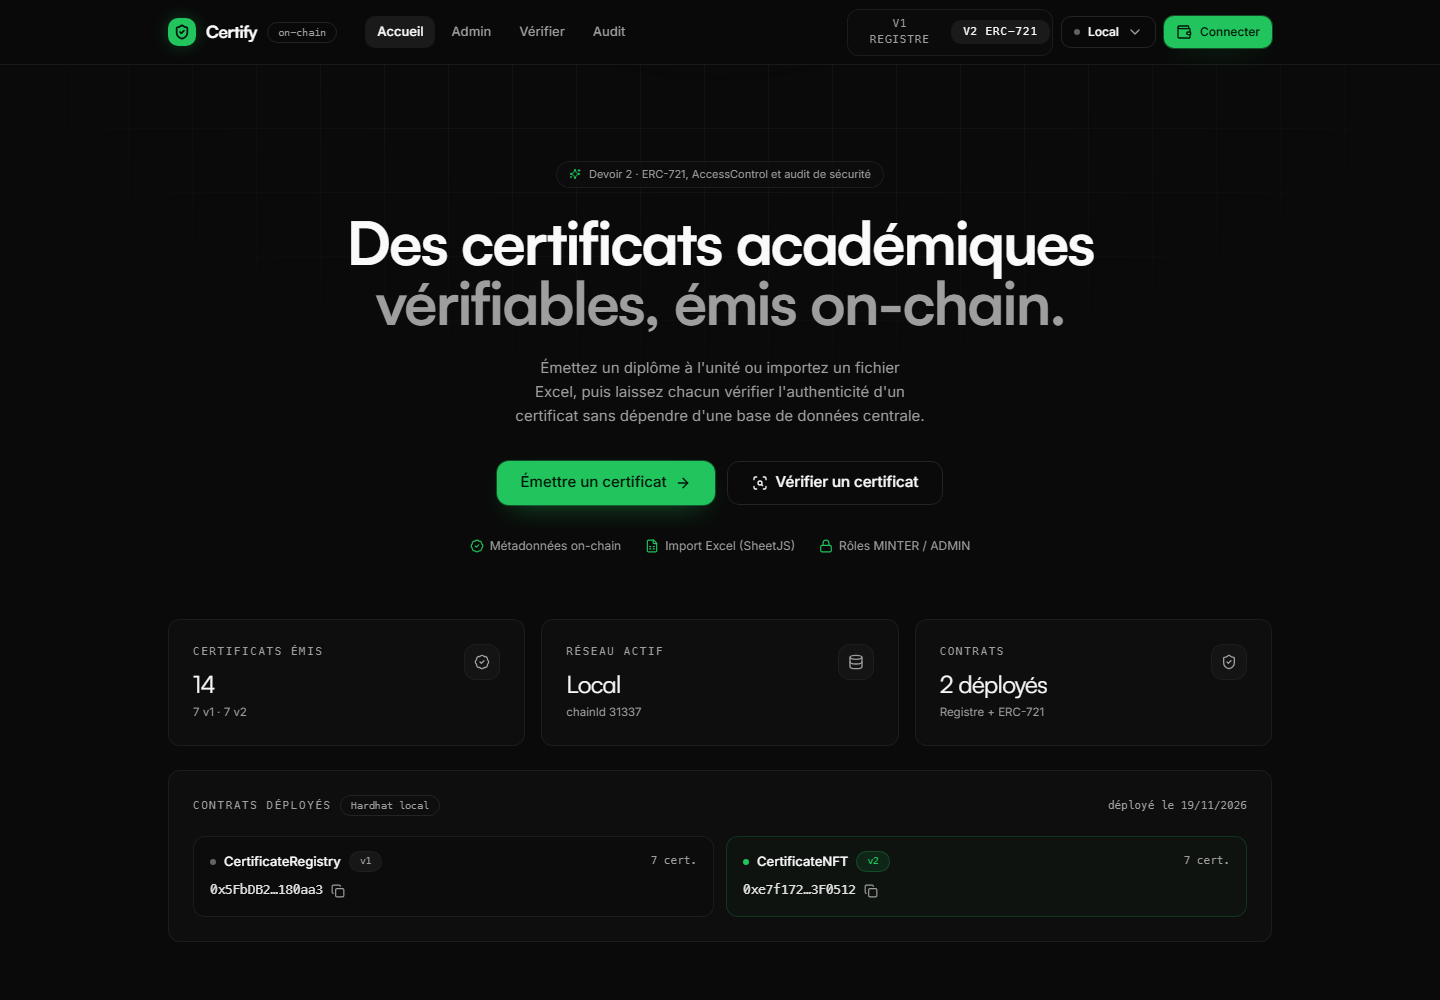
\includegraphics[width=0.92\textwidth]{01-accueil.png}
\caption{Sélecteur de version et compteurs des deux contrats.}
\label{fig:home}
\end{figure}

\begin{figure}[htbp]
\centering
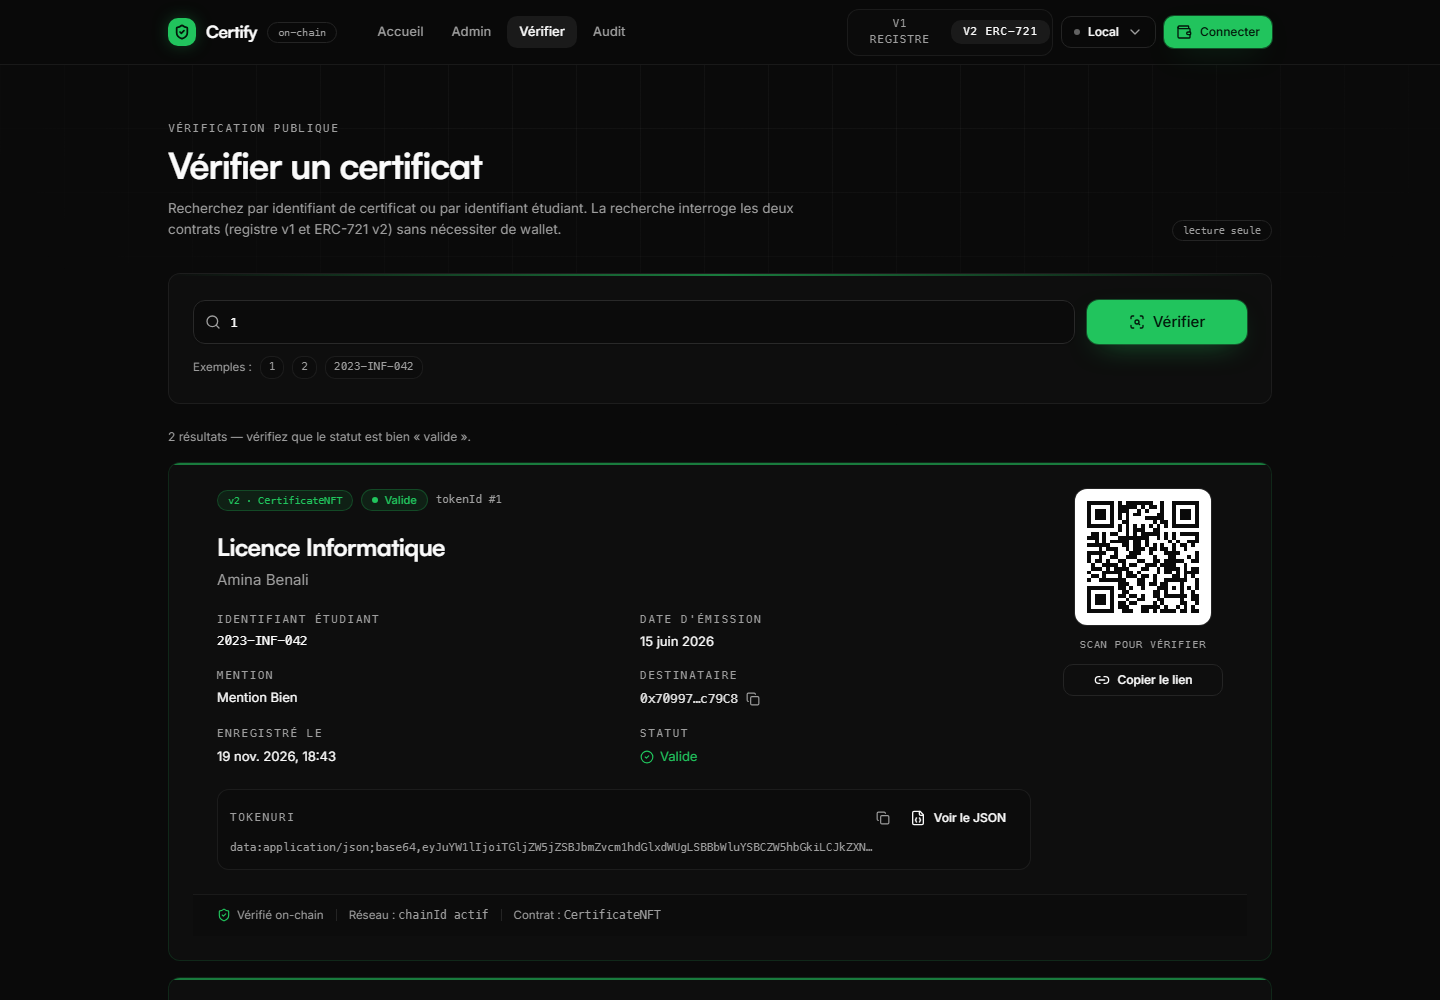
\includegraphics[width=0.92\textwidth]{03-verify-id.png}
\caption{Vérification du certificat \texttt{\#1} et décodage des métadonnées.}
\label{fig:token}
\end{figure}

\section{Ce qui reste ouvert}

\begin{itemize}
\item Borner la taille des métadonnées, ou déporter les données lourdes vers IPFS
  en ne gardant qu'un hash on-chain.
\item Documenter la forme canonique du \texttt{studentId} et centraliser
  l'émission, pour éviter deux variantes d'un même identifiant.
\item Séparer la révocation de l'administration avec un rôle dédié, puis placer
  le rôle admin dans un Safe.
\item Ajouter un indexeur pour l'historique complet des événements, et déployer
  sur Sepolia avec vérification du code avant toute démonstration publique.
\end{itemize}

\section{Pour relancer}

\begin{lstlisting}[basicstyle=\ttfamily\small]
cd certificats
npm install
npm run node           # terminal 1
npm run deploy:local   # terminal 2
npm run seed:local
npm run smoke:local
npm run dev            # terminal 3
\end{lstlisting}

\end{document}
